\documentclass[twoside]{book}

% Packages required by doxygen
\usepackage{fixltx2e}
\usepackage{calc}
\usepackage{doxygen}
\usepackage[export]{adjustbox} % also loads graphicx
\usepackage{graphicx}
\usepackage[utf8]{inputenc}
\usepackage{makeidx}
\usepackage{multicol}
\usepackage{multirow}
\PassOptionsToPackage{warn}{textcomp}
\usepackage{textcomp}
\usepackage[nointegrals]{wasysym}
\usepackage[table]{xcolor}

% Font selection
\usepackage[T1]{fontenc}
\usepackage[scaled=.90]{helvet}
\usepackage{courier}
\usepackage{amssymb}
\usepackage{sectsty}
\renewcommand{\familydefault}{\sfdefault}
\allsectionsfont{%
  \fontseries{bc}\selectfont%
  \color{darkgray}%
}
\renewcommand{\DoxyLabelFont}{%
  \fontseries{bc}\selectfont%
  \color{darkgray}%
}
\newcommand{\+}{\discretionary{\mbox{\scriptsize$\hookleftarrow$}}{}{}}

% Page & text layout
\usepackage{geometry}
\geometry{%
  a4paper,%
  top=2.5cm,%
  bottom=2.5cm,%
  left=2.5cm,%
  right=2.5cm%
}
\tolerance=750
\hfuzz=15pt
\hbadness=750
\setlength{\emergencystretch}{15pt}
\setlength{\parindent}{0cm}
\setlength{\parskip}{3ex plus 2ex minus 2ex}
\makeatletter
\renewcommand{\paragraph}{%
  \@startsection{paragraph}{4}{0ex}{-1.0ex}{1.0ex}{%
    \normalfont\normalsize\bfseries\SS@parafont%
  }%
}
\renewcommand{\subparagraph}{%
  \@startsection{subparagraph}{5}{0ex}{-1.0ex}{1.0ex}{%
    \normalfont\normalsize\bfseries\SS@subparafont%
  }%
}
\makeatother

% Headers & footers
\usepackage{fancyhdr}
\pagestyle{fancyplain}
\fancyhead[LE]{\fancyplain{}{\bfseries\thepage}}
\fancyhead[CE]{\fancyplain{}{}}
\fancyhead[RE]{\fancyplain{}{\bfseries\leftmark}}
\fancyhead[LO]{\fancyplain{}{\bfseries\rightmark}}
\fancyhead[CO]{\fancyplain{}{}}
\fancyhead[RO]{\fancyplain{}{\bfseries\thepage}}
\fancyfoot[LE]{\fancyplain{}{}}
\fancyfoot[CE]{\fancyplain{}{}}
\fancyfoot[RE]{\fancyplain{}{\bfseries\scriptsize Generated by Doxygen }}
\fancyfoot[LO]{\fancyplain{}{\bfseries\scriptsize Generated by Doxygen }}
\fancyfoot[CO]{\fancyplain{}{}}
\fancyfoot[RO]{\fancyplain{}{}}
\renewcommand{\footrulewidth}{0.4pt}
\renewcommand{\chaptermark}[1]{%
  \markboth{#1}{}%
}
\renewcommand{\sectionmark}[1]{%
  \markright{\thesection\ #1}%
}

% Indices & bibliography
\usepackage{natbib}
\usepackage[titles]{tocloft}
\setcounter{tocdepth}{3}
\setcounter{secnumdepth}{5}
\makeindex

% Hyperlinks (required, but should be loaded last)
\usepackage{ifpdf}
\ifpdf
  \usepackage[pdftex,pagebackref=true]{hyperref}
\else
  \usepackage[ps2pdf,pagebackref=true]{hyperref}
\fi
\hypersetup{%
  colorlinks=true,%
  linkcolor=blue,%
  citecolor=blue,%
  unicode%
}

% Custom commands
\newcommand{\clearemptydoublepage}{%
  \newpage{\pagestyle{empty}\cleardoublepage}%
}

\usepackage{caption}
\captionsetup{labelsep=space,justification=centering,font={bf},singlelinecheck=off,skip=4pt,position=top}

%===== C O N T E N T S =====

\begin{document}

% Titlepage & ToC
\hypersetup{pageanchor=false,
             bookmarksnumbered=true,
             pdfencoding=unicode
            }
\pagenumbering{roman}
\begin{titlepage}
\vspace*{7cm}
\begin{center}%
{\Large Nouveau Analysis \\[1ex]\large 0.\+1 }\\
\vspace*{1cm}
{\large Generated by Doxygen 1.8.11}\\
\end{center}
\end{titlepage}
\clearemptydoublepage
\tableofcontents
\clearemptydoublepage
\pagenumbering{arabic}
\hypersetup{pageanchor=true}

%--- Begin generated contents ---
\chapter{Hierarchical Index}
\section{Class Hierarchy}
This inheritance list is sorted roughly, but not completely, alphabetically\+:\begin{DoxyCompactList}
\item \contentsline{section}{Flat\+File\+Reader}{\pageref{class_flat_file_reader}}{}
\begin{DoxyCompactList}
\item \contentsline{section}{Flat\+File\+Parser}{\pageref{class_flat_file_parser}}{}
\end{DoxyCompactList}
\item \contentsline{section}{Flat\+File\+Saver}{\pageref{class_flat_file_saver}}{}
\item \contentsline{section}{K\+S\+V\+Z\+Power\+Spec}{\pageref{class_k_s_v_z_power_spec}}{}
\item \contentsline{section}{Single\+Spectrum}{\pageref{class_single_spectrum}}{}
\item \contentsline{section}{Spectrum}{\pageref{class_spectrum}}{}
\item \contentsline{section}{Spectrum\+Parameters}{\pageref{struct_spectrum_parameters}}{}
\end{DoxyCompactList}

\chapter{Class Index}
\section{Class List}
Here are the classes, structs, unions and interfaces with brief descriptions\+:\begin{DoxyCompactList}
\item\contentsline{section}{\hyperlink{class_flat_file_parser}{Flat\+File\+Parser} }{\pageref{class_flat_file_parser}}{}
\item\contentsline{section}{\hyperlink{class_flat_file_reader}{Flat\+File\+Reader} }{\pageref{class_flat_file_reader}}{}
\item\contentsline{section}{\hyperlink{class_flat_file_saver}{Flat\+File\+Saver} }{\pageref{class_flat_file_saver}}{}
\item\contentsline{section}{\hyperlink{class_k_s_v_z_power_spec}{K\+S\+V\+Z\+Power\+Spec} }{\pageref{class_k_s_v_z_power_spec}}{}
\item\contentsline{section}{\hyperlink{class_single_spectrum}{Single\+Spectrum} \\*Class to hold a single power spectrum and its associated parameters, such as center frequency, frequency span, Q etc }{\pageref{class_single_spectrum}}{}
\item\contentsline{section}{\hyperlink{class_spectrum}{Spectrum} }{\pageref{class_spectrum}}{}
\item\contentsline{section}{\hyperlink{struct_spectrum_parameters}{Spectrum\+Parameters} }{\pageref{struct_spectrum_parameters}}{}
\end{DoxyCompactList}

\chapter{Class Documentation}
\hypertarget{class_flat_file_parser}{}\section{Flat\+File\+Parser Class Reference}
\label{class_flat_file_parser}\index{Flat\+File\+Parser@{Flat\+File\+Parser}}
Inheritance diagram for Flat\+File\+Parser\+:\begin{figure}[H]
\begin{center}
\leavevmode
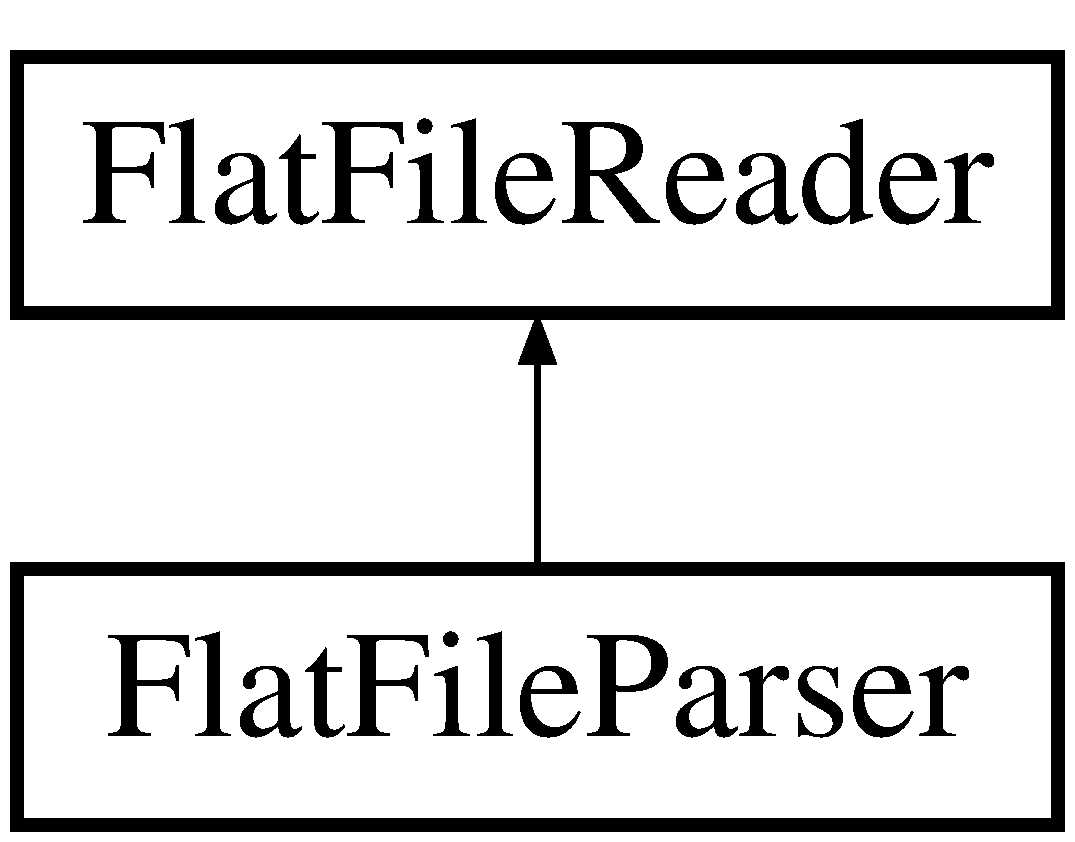
\includegraphics[height=2.000000cm]{class_flat_file_parser}
\end{center}
\end{figure}
\subsection*{Public Member Functions}
\begin{DoxyCompactItemize}
\item 
{\bfseries Flat\+File\+Parser} (std\+::string raw\+\_\+data)\hypertarget{class_flat_file_parser_a5b1d9499abae7dcd01aff8310aa2cbac}{}\label{class_flat_file_parser_a5b1d9499abae7dcd01aff8310aa2cbac}

\item 
std\+::vector$<$ double $>$ {\bfseries Get\+Power\+List} ()\hypertarget{class_flat_file_parser_a89a4dbb69920e61263da9b0ff410f4fc}{}\label{class_flat_file_parser_a89a4dbb69920e61263da9b0ff410f4fc}

\item 
std\+::map$<$ std\+::string, double $>$ {\bfseries Get\+Header} ()\hypertarget{class_flat_file_parser_aa800cd7f2868c1635cf85475380fad14}{}\label{class_flat_file_parser_aa800cd7f2868c1635cf85475380fad14}

\end{DoxyCompactItemize}


\subsection{Detailed Description}


Definition at line 40 of file flatfileinterface.\+h.


\hypertarget{class_flat_file_reader}{}\section{Flat\+File\+Reader Class Reference}
\label{class_flat_file_reader}\index{Flat\+File\+Reader@{Flat\+File\+Reader}}
Inheritance diagram for Flat\+File\+Reader\+:\begin{figure}[H]
\begin{center}
\leavevmode
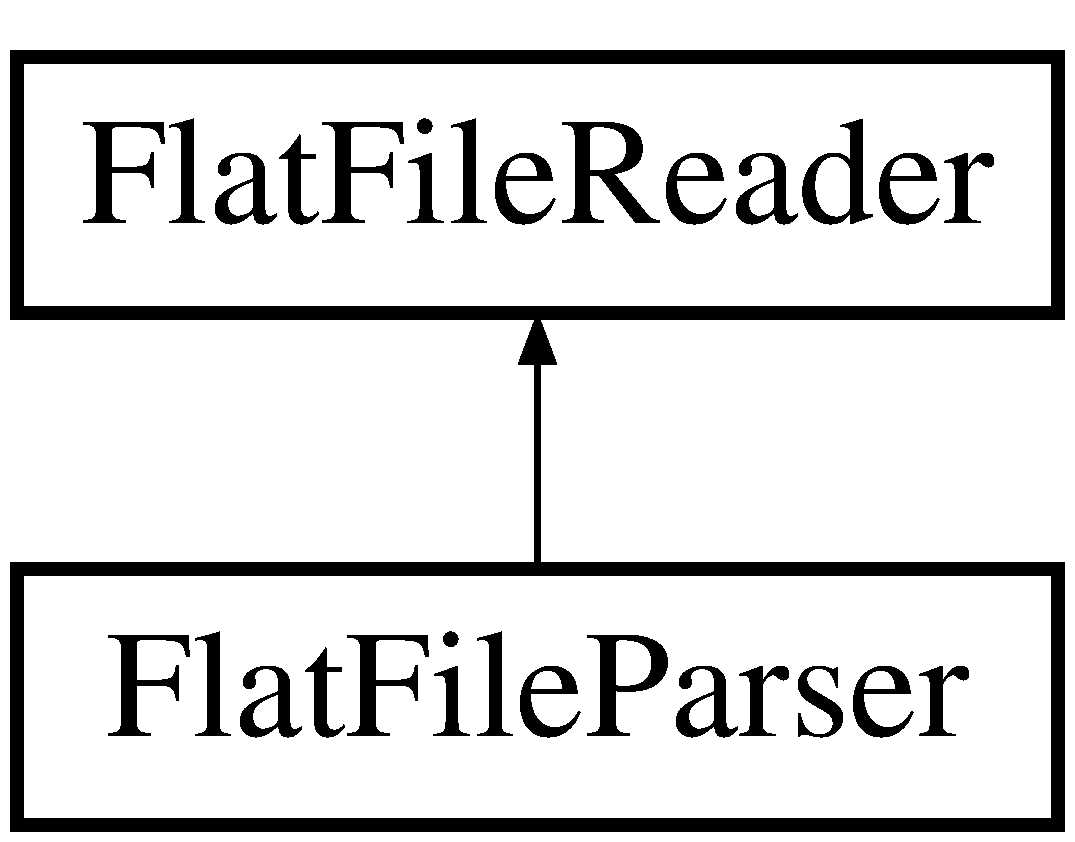
\includegraphics[height=2.000000cm]{class_flat_file_reader}
\end{center}
\end{figure}
\subsection*{Public Member Functions}
\begin{DoxyCompactItemize}
\item 
{\bfseries Flat\+File\+Reader} (std\+::string dir\+\_\+name)\hypertarget{class_flat_file_reader_ae1c5000a285394231a542c2eabf09b85}{}\label{class_flat_file_reader_ae1c5000a285394231a542c2eabf09b85}

\item 
std\+::string {\bfseries at} (uint index)\hypertarget{class_flat_file_reader_aa743c454c716503a9b77368dced7d86c}{}\label{class_flat_file_reader_aa743c454c716503a9b77368dced7d86c}

\item 
uint {\bfseries size} ()\hypertarget{class_flat_file_reader_ae384eb0fdcbbf2b6e6a666761ad9767a}{}\label{class_flat_file_reader_ae384eb0fdcbbf2b6e6a666761ad9767a}

\item 
bool {\bfseries has} (uint index)\hypertarget{class_flat_file_reader_ad0c541a53501a7310ff1294c815c3e29}{}\label{class_flat_file_reader_ad0c541a53501a7310ff1294c815c3e29}

\end{DoxyCompactItemize}


\subsection{Detailed Description}


Definition at line 19 of file flatfileinterface.\+h.


\hypertarget{class_flat_file_saver}{}\section{Flat\+File\+Saver Class Reference}
\label{class_flat_file_saver}\index{Flat\+File\+Saver@{Flat\+File\+Saver}}
\subsection*{Public Member Functions}
\begin{DoxyCompactItemize}
\item 
{\bfseries Flat\+File\+Saver} (std\+::string dir\+\_\+name)\hypertarget{class_flat_file_saver_a1778a44559f342a2c102842a58c9866b}{}\label{class_flat_file_saver_a1778a44559f342a2c102842a58c9866b}

\item 
{\footnotesize template$<$typename T $>$ }\\void {\bfseries load} (std\+::map$<$ std\+::string, T $>$ header)\hypertarget{class_flat_file_saver_a8914a6ba17ea3b6e4891af8138b518bb}{}\label{class_flat_file_saver_a8914a6ba17ea3b6e4891af8138b518bb}

\item 
{\footnotesize template$<$typename T $>$ }\\void {\bfseries load} (std\+::vector$<$ T $>$ vec)\hypertarget{class_flat_file_saver_a7b14fc970538db6d07fc132c212b3225}{}\label{class_flat_file_saver_a7b14fc970538db6d07fc132c212b3225}

\item 
bool {\bfseries dump} ()\hypertarget{class_flat_file_saver_af7b235135124fe78ec3f60d531ea9200}{}\label{class_flat_file_saver_af7b235135124fe78ec3f60d531ea9200}

\end{DoxyCompactItemize}


\subsection{Detailed Description}


Definition at line 56 of file flatfileinterface.\+h.


\hypertarget{class_k_s_v_z_power_spec}{}\section{K\+S\+V\+Z\+Power\+Spec Class Reference}
\label{class_k_s_v_z_power_spec}\index{K\+S\+V\+Z\+Power\+Spec@{K\+S\+V\+Z\+Power\+Spec}}


\subsection{Detailed Description}


Definition at line 133 of file spectrum.\+h.


\hypertarget{class_single_spectrum}{}\section{Single\+Spectrum Class Reference}
\label{class_single_spectrum}\index{Single\+Spectrum@{Single\+Spectrum}}


Class to hold a single power spectrum and its associated parameters, such as center frequency, frequency span, Q etc.  




{\ttfamily \#include $<$spectrum.\+h$>$}

\subsection*{Public Member Functions}
\begin{DoxyCompactItemize}
\item 
{\bfseries Single\+Spectrum} (std\+::string raw\+\_\+data)\hypertarget{class_single_spectrum_a4a3601f0303e217a3b58458d5f47c05a}{}\label{class_single_spectrum_a4a3601f0303e217a3b58458d5f47c05a}

\item 
{\bfseries Single\+Spectrum} (uint size)\hypertarget{class_single_spectrum_a964a944ac1fa20c59d18a1aec62ac149}{}\label{class_single_spectrum_a964a944ac1fa20c59d18a1aec62ac149}

\item 
\hyperlink{class_single_spectrum}{Single\+Spectrum} \& {\bfseries operator$\ast$=} (double scalar)\hypertarget{class_single_spectrum_a1036113bfa175f06d75b6b5b0607a41d}{}\label{class_single_spectrum_a1036113bfa175f06d75b6b5b0607a41d}

\item 
\hyperlink{class_single_spectrum}{Single\+Spectrum} \& {\bfseries operator+=} (double scalar)\hypertarget{class_single_spectrum_a324cc374d07ca086f435e8f917eda9ed}{}\label{class_single_spectrum_a324cc374d07ca086f435e8f917eda9ed}

\item 
void {\bfseries Normalize} ()\hypertarget{class_single_spectrum_a938eb09122d2775378a4e100ee8717f4}{}\label{class_single_spectrum_a938eb09122d2775378a4e100ee8717f4}

\item 
double {\bfseries std\+\_\+dev} ()\hypertarget{class_single_spectrum_a138e3db04f9db67a699c8dddfef8f324}{}\label{class_single_spectrum_a138e3db04f9db67a699c8dddfef8f324}

\item 
double {\bfseries mean} ()\hypertarget{class_single_spectrum_a39f66345fd7d6502bbc8ba731cc1bb13}{}\label{class_single_spectrum_a39f66345fd7d6502bbc8ba731cc1bb13}

\item 
uint {\bfseries size} ()\hypertarget{class_single_spectrum_a42c2d13e632ffc2d4f0931376c5b6e5b}{}\label{class_single_spectrum_a42c2d13e632ffc2d4f0931376c5b6e5b}

\item 
void {\bfseries rebin} (uint points\+\_\+per\+\_\+bin)\hypertarget{class_single_spectrum_ac39957d9b67a322272d1089aa6dd6c4c}{}\label{class_single_spectrum_ac39957d9b67a322272d1089aa6dd6c4c}

\item 
void {\bfseries chop\+\_\+bins} (uint start\+\_\+chop, uint end\+\_\+chop)\hypertarget{class_single_spectrum_afea78595e8232ecb15f3c2f5d825cef1}{}\label{class_single_spectrum_afea78595e8232ecb15f3c2f5d825cef1}

\item 
double {\bfseries bin\+\_\+start\+\_\+freq} (uint idx)\hypertarget{class_single_spectrum_a2bda515f49feea97f76bd06f441a9c2d}{}\label{class_single_spectrum_a2bda515f49feea97f76bd06f441a9c2d}

\item 
double {\bfseries bin\+\_\+mid\+\_\+freq} (uint idx)\hypertarget{class_single_spectrum_a0a1e03366e1b482decd42326187cdcf5}{}\label{class_single_spectrum_a0a1e03366e1b482decd42326187cdcf5}

\item 
double {\bfseries bin\+\_\+width} ()\hypertarget{class_single_spectrum_aad6dfbabe270fbc5ac7ce0dafdb77197}{}\label{class_single_spectrum_aad6dfbabe270fbc5ac7ce0dafdb77197}

\item 
double {\bfseries kszv\+\_\+power\+\_\+per\+\_\+bin} (double freq\+\_\+mhz)\hypertarget{class_single_spectrum_a9944b692eebbb9e032a4ce44f63c37fe}{}\label{class_single_spectrum_a9944b692eebbb9e032a4ce44f63c37fe}

\item 
uint {\bfseries bin\+\_\+at\+\_\+frequency} (double frequency)\hypertarget{class_single_spectrum_a98378d6007966e7706624f55ea35b975}{}\label{class_single_spectrum_a98378d6007966e7706624f55ea35b975}

\end{DoxyCompactItemize}
\subsection*{Protected Attributes}
\begin{DoxyCompactItemize}
\item 
std\+::vector$<$ double $>$ {\bfseries sa\+\_\+power\+\_\+list}\hypertarget{class_single_spectrum_a5aca204ca152d33748820e473955a1b0}{}\label{class_single_spectrum_a5aca204ca152d33748820e473955a1b0}

\item 
std\+::vector$<$ double $>$ {\bfseries uncertainties}\hypertarget{class_single_spectrum_ad2c19bf0653a56f7d21709f5b8796b67}{}\label{class_single_spectrum_ad2c19bf0653a56f7d21709f5b8796b67}

\end{DoxyCompactItemize}
\subsection*{Friends}
\begin{DoxyCompactItemize}
\item 
bool {\bfseries operator==} (\hyperlink{class_single_spectrum}{Single\+Spectrum} \&spectra\+\_\+a, \hyperlink{class_single_spectrum}{Single\+Spectrum} \&spectra\+\_\+b)\hypertarget{class_single_spectrum_a6ba91d2d92db2828951645e19e0a0384}{}\label{class_single_spectrum_a6ba91d2d92db2828951645e19e0a0384}

\item 
bool {\bfseries operator!=} (\hyperlink{class_single_spectrum}{Single\+Spectrum} \&spectra\+\_\+a, \hyperlink{class_single_spectrum}{Single\+Spectrum} \&spectra\+\_\+b)\hypertarget{class_single_spectrum_ae0a9f33112a5508cf8d5613a165c11df}{}\label{class_single_spectrum_ae0a9f33112a5508cf8d5613a165c11df}

\item 
std\+::ostream \& \hyperlink{class_single_spectrum_a260e8ff3518714d32d964dd7e2a6bf39}{operator$<$$<$} (std\+::ostream \&stream, \hyperlink{class_single_spectrum}{Single\+Spectrum} \&spectrum)
\begin{DoxyCompactList}\small\item\em Operator for printing spectrum contents to std\+::cout or similar Only power data will be accessed and printed. \end{DoxyCompactList}\item 
std\+::ofstream \& \hyperlink{class_single_spectrum_aa4fcc146ff71fd379f2e6dab83125c74}{operator$<$$<$} (std\+::ofstream \&stream, \hyperlink{class_single_spectrum}{Single\+Spectrum} \&spectrum)
\begin{DoxyCompactList}\small\item\em Operator for saving spectra to files Unlike the ostream version, both the header and power data are accessed. \end{DoxyCompactList}\item 
\hyperlink{class_single_spectrum}{Single\+Spectrum} {\bfseries operator$\ast$} (\hyperlink{class_single_spectrum}{Single\+Spectrum} \&spectra\+\_\+a, \hyperlink{class_single_spectrum}{Single\+Spectrum} \&spectra\+\_\+b)\hypertarget{class_single_spectrum_ac71261d3ce99c4028fae4996736a72b3}{}\label{class_single_spectrum_ac71261d3ce99c4028fae4996736a72b3}

\item 
\hyperlink{class_single_spectrum}{Single\+Spectrum} {\bfseries operator+} (\hyperlink{class_single_spectrum}{Single\+Spectrum} \&spectra\+\_\+a, \hyperlink{class_single_spectrum}{Single\+Spectrum} \&spectra\+\_\+b)\hypertarget{class_single_spectrum_aff381ffcc9205b4b376b6af20c6bd98d}{}\label{class_single_spectrum_aff381ffcc9205b4b376b6af20c6bd98d}

\item 
\hyperlink{class_single_spectrum}{Single\+Spectrum} {\bfseries operator-\/} (\hyperlink{class_single_spectrum}{Single\+Spectrum} \&spectra\+\_\+a, \hyperlink{class_single_spectrum}{Single\+Spectrum} \&spectra\+\_\+b)\hypertarget{class_single_spectrum_a323a1a48dc567b58ac1a4ef41ddd06c7}{}\label{class_single_spectrum_a323a1a48dc567b58ac1a4ef41ddd06c7}

\item 
\hyperlink{class_single_spectrum}{Single\+Spectrum} {\bfseries operator$\ast$} (\hyperlink{class_single_spectrum}{Single\+Spectrum} \&spectra\+\_\+a, std\+::vector$<$ double $>$ \&spectra\+\_\+b)\hypertarget{class_single_spectrum_a03a486faf7f42ef4c5e407cf510a8ac8}{}\label{class_single_spectrum_a03a486faf7f42ef4c5e407cf510a8ac8}

\item 
\hyperlink{class_single_spectrum}{Single\+Spectrum} {\bfseries operator+} (\hyperlink{class_single_spectrum}{Single\+Spectrum} \&spectra\+\_\+a, std\+::vector$<$ double $>$ \&spectra\+\_\+b)\hypertarget{class_single_spectrum_a94b2bcfa34d2a268cf575ed0310f9862}{}\label{class_single_spectrum_a94b2bcfa34d2a268cf575ed0310f9862}

\item 
\hyperlink{class_single_spectrum}{Single\+Spectrum} {\bfseries operator-\/} (\hyperlink{class_single_spectrum}{Single\+Spectrum} \&spectra\+\_\+a, std\+::vector$<$ double $>$ \&spectra\+\_\+b)\hypertarget{class_single_spectrum_af09eb1e4819bdc296e86ae5184801c15}{}\label{class_single_spectrum_af09eb1e4819bdc296e86ae5184801c15}

\item 
void \hyperlink{class_single_spectrum_a50289b4319d5367695533d6a92833109}{To\+Watts\+Above\+Noise} (\hyperlink{class_single_spectrum}{Single\+Spectrum} \&spectra\+\_\+a)\hypertarget{class_single_spectrum_a50289b4319d5367695533d6a92833109}{}\label{class_single_spectrum_a50289b4319d5367695533d6a92833109}

\begin{DoxyCompactList}\small\item\em Convert from usings of d\+Bm to units of watts above noise (i.\+e. excess power) \end{DoxyCompactList}\end{DoxyCompactItemize}


\subsection{Detailed Description}
Class to hold a single power spectrum and its associated parameters, such as center frequency, frequency span, Q etc. 

Class is designed to \textquotesingle{}look and feel\textquotesingle{} like a $ \mathcal{R}^n $ vector. Spectra allows scalar multiplication and addition, along with \textquotesingle{}vector\textquotesingle{} multiplication and addition. 

Definition at line 39 of file spectrum.\+h.



\subsection{Friends And Related Function Documentation}
\index{Single\+Spectrum@{Single\+Spectrum}!operator$<$$<$@{operator$<$$<$}}
\index{operator$<$$<$@{operator$<$$<$}!Single\+Spectrum@{Single\+Spectrum}}
\subsubsection[{\texorpdfstring{operator$<$$<$}{operator<<}}]{\setlength{\rightskip}{0pt plus 5cm}std\+::ostream\& operator$<$$<$ (
\begin{DoxyParamCaption}
\item[{std\+::ostream \&}]{stream, }
\item[{{\bf Single\+Spectrum} \&}]{spectrum}
\end{DoxyParamCaption}
)\hspace{0.3cm}{\ttfamily [friend]}}\hypertarget{class_single_spectrum_a260e8ff3518714d32d964dd7e2a6bf39}{}\label{class_single_spectrum_a260e8ff3518714d32d964dd7e2a6bf39}


Operator for printing spectrum contents to std\+::cout or similar Only power data will be accessed and printed. 


\begin{DoxyParams}{Parameters}
{\em stream} & object \\
\hline
{\em spectrum} & to be printed \\
\hline
\end{DoxyParams}
\begin{DoxyReturn}{Returns}
new stream object 
\end{DoxyReturn}


Definition at line 84 of file spectrum.\+cpp.

\index{Single\+Spectrum@{Single\+Spectrum}!operator$<$$<$@{operator$<$$<$}}
\index{operator$<$$<$@{operator$<$$<$}!Single\+Spectrum@{Single\+Spectrum}}
\subsubsection[{\texorpdfstring{operator$<$$<$}{operator<<}}]{\setlength{\rightskip}{0pt plus 5cm}std\+::ofstream\& operator$<$$<$ (
\begin{DoxyParamCaption}
\item[{std\+::ofstream \&}]{stream, }
\item[{{\bf Single\+Spectrum} \&}]{spectrum}
\end{DoxyParamCaption}
)\hspace{0.3cm}{\ttfamily [friend]}}\hypertarget{class_single_spectrum_aa4fcc146ff71fd379f2e6dab83125c74}{}\label{class_single_spectrum_aa4fcc146ff71fd379f2e6dab83125c74}


Operator for saving spectra to files Unlike the ostream version, both the header and power data are accessed. 


\begin{DoxyParams}{Parameters}
{\em stream} & object \\
\hline
{\em spectrum} & to be saved \\
\hline
\end{DoxyParams}
\begin{DoxyReturn}{Returns}
new stream object 
\end{DoxyReturn}


Definition at line 93 of file spectrum.\+cpp.


\hypertarget{class_spectrum}{}\section{Spectrum Class Reference}
\label{class_spectrum}\index{Spectrum@{Spectrum}}
\subsection*{Public Member Functions}
\begin{DoxyCompactItemize}
\item 
\hyperlink{class_spectrum}{Spectrum} \& {\bfseries operator+=} (\hyperlink{class_single_spectrum}{Single\+Spectrum} \&spec)\hypertarget{class_spectrum_ac30c829d8ae1bdde1a0ea0e6cef87a4d}{}\label{class_spectrum_ac30c829d8ae1bdde1a0ea0e6cef87a4d}

\item 
\hyperlink{class_spectrum}{Spectrum} \& {\bfseries operator-\/=} (\hyperlink{class_single_spectrum}{Single\+Spectrum} \&spec)\hypertarget{class_spectrum_a811119db4a9a80559d48e4515a6459b8}{}\label{class_spectrum_a811119db4a9a80559d48e4515a6459b8}

\item 
\hyperlink{class_single_spectrum}{Single\+Spectrum} {\bfseries Grand\+Spectrum} ()\hypertarget{class_spectrum_a041b82b8cc88be4f8d701aa3fac066e6}{}\label{class_spectrum_a041b82b8cc88be4f8d701aa3fac066e6}

\item 
\hyperlink{class_single_spectrum}{Single\+Spectrum} {\bfseries Limits} ()\hypertarget{class_spectrum_a14abc191ca8f12552a54b6bb09567fb5}{}\label{class_spectrum_a14abc191ca8f12552a54b6bb09567fb5}

\item 
uint {\bfseries size} ()\hypertarget{class_spectrum_a9640391cdb12174df3e816f4cc74adec}{}\label{class_spectrum_a9640391cdb12174df3e816f4cc74adec}

\item 
void {\bfseries clear} ()\hypertarget{class_spectrum_ad62a0ee86cfe3eb5a0c29069174a5129}{}\label{class_spectrum_ad62a0ee86cfe3eb5a0c29069174a5129}

\end{DoxyCompactItemize}


\subsection{Detailed Description}


Definition at line 143 of file spectrum.\+h.


\hypertarget{struct_spectrum_parameters}{}\section{Spectrum\+Parameters Struct Reference}
\label{struct_spectrum_parameters}\index{Spectrum\+Parameters@{Spectrum\+Parameters}}
\subsection*{Public Attributes}
\begin{DoxyCompactItemize}
\item 
double {\bfseries center\+\_\+frequency} = 0.\+0\hypertarget{struct_spectrum_parameters_a56975b921e499f10c9fb4c08ba828547}{}\label{struct_spectrum_parameters_a56975b921e499f10c9fb4c08ba828547}

\item 
double {\bfseries frequency\+\_\+span} = 0.\+0\hypertarget{struct_spectrum_parameters_a2941b715e103c34a0356f4ee49745567}{}\label{struct_spectrum_parameters_a2941b715e103c34a0356f4ee49745567}

\item 
double {\bfseries effective\+\_\+volume} = 0.\+0\hypertarget{struct_spectrum_parameters_a2c0a77f3fa260127a17376041e5fe109}{}\label{struct_spectrum_parameters_a2c0a77f3fa260127a17376041e5fe109}

\item 
double {\bfseries Q} = 0.\+0\hypertarget{struct_spectrum_parameters_a753173b3591c797a15b8d536eef4c7f8}{}\label{struct_spectrum_parameters_a753173b3591c797a15b8d536eef4c7f8}

\item 
uint {\bfseries number\+\_\+of\+\_\+averages} = 0\hypertarget{struct_spectrum_parameters_afa3f30ba0906616b6e0bfb4c7b326806}{}\label{struct_spectrum_parameters_afa3f30ba0906616b6e0bfb4c7b326806}

\item 
uint {\bfseries fft\+\_\+points} = 0\hypertarget{struct_spectrum_parameters_a4cb7ebf7f023c2c82ccfd888da3e5ff3}{}\label{struct_spectrum_parameters_a4cb7ebf7f023c2c82ccfd888da3e5ff3}

\end{DoxyCompactItemize}


\subsection{Detailed Description}


Definition at line 20 of file spectrum.\+h.


%--- End generated contents ---

% Index
\backmatter
\newpage
\phantomsection
\clearemptydoublepage
\addcontentsline{toc}{chapter}{Index}
\printindex

\end{document}
